% !TeX spellcheck = da_DK
\subsection{Spændingsforsyning}
\subsubsection{Teori og design}
Til systemet anvendes to $1.5$V batterier som spændingsforsyning, der sidder i en spændingsregulator. Denne kan leverer en spænding på $\pm5.5$V og $\pm3.3$V fra to forskellige terminaler. Derudover besidder spændingsregulatoren en jordkobling, som øvrige komponenter i systemet kan kobles til. I dette projekt benyttes terminalalen med en spændingen på $\pm5.5$V. Spændingsregulatoren er designet således, at den leverer en spænding koblet i et splitsupply. Spændingsregulatorens negative spændingsforsyning kaldes $-V_{cc}$ og den positive kaldes $+V_{cc}$. \\%Den positive pol fra det ene batteri tilkobles den negative pol på det andet batteri i. Derudover dannes en fælles jordforbindelse for øvrige komponenter i systemet, som kræver en forbindelse til jord. Den negative pol i det første batteri i det første batteri anvendes som systemets negative forsyningsspænding og indikeres med $-V_{cc}$, mens det andet batteri anvendes som den positive spændingsforsyning og indikeres med $+V_{cc}$.
Da batterierne ikke leverer den samme spænding over hele batteriernes levetid, skal batteriet skiftes ud, når de ikke leverer den nødvendige spænding til systemet. Batteriernes levetid afhænger af, hvor meget strøm systemet trækker. %Da komparatorkonfigurationen kræver den højeste spænding iblandt blokkene, skal spændingsregulatoren minimum leverer en spænding på xx V. Derfor kræver systemt en minimal spænding på xx V.

\subsubsection{Simulering}
Ved simulering af spændingsforsyningen anvendes LTspice, hvor der simuleres en spænding igennem en buffer, som også er beskrevet og benyttet i afsnit \ref{Offset_Teori_Design} på side \pageref{Offset_Teori_Design}. Herved kan konsekvensen af et faldende input simuleres. Der undersøges flere forskellige spændinger ved at ændre på spændingsforsyningen, hvilket er illustreret på \figref{fig:spaendingsforsyning}. Der undersøges for hhv. $5$V, $4.5$V og $4.3$V.
\begin{figure}[H]
	\centering
	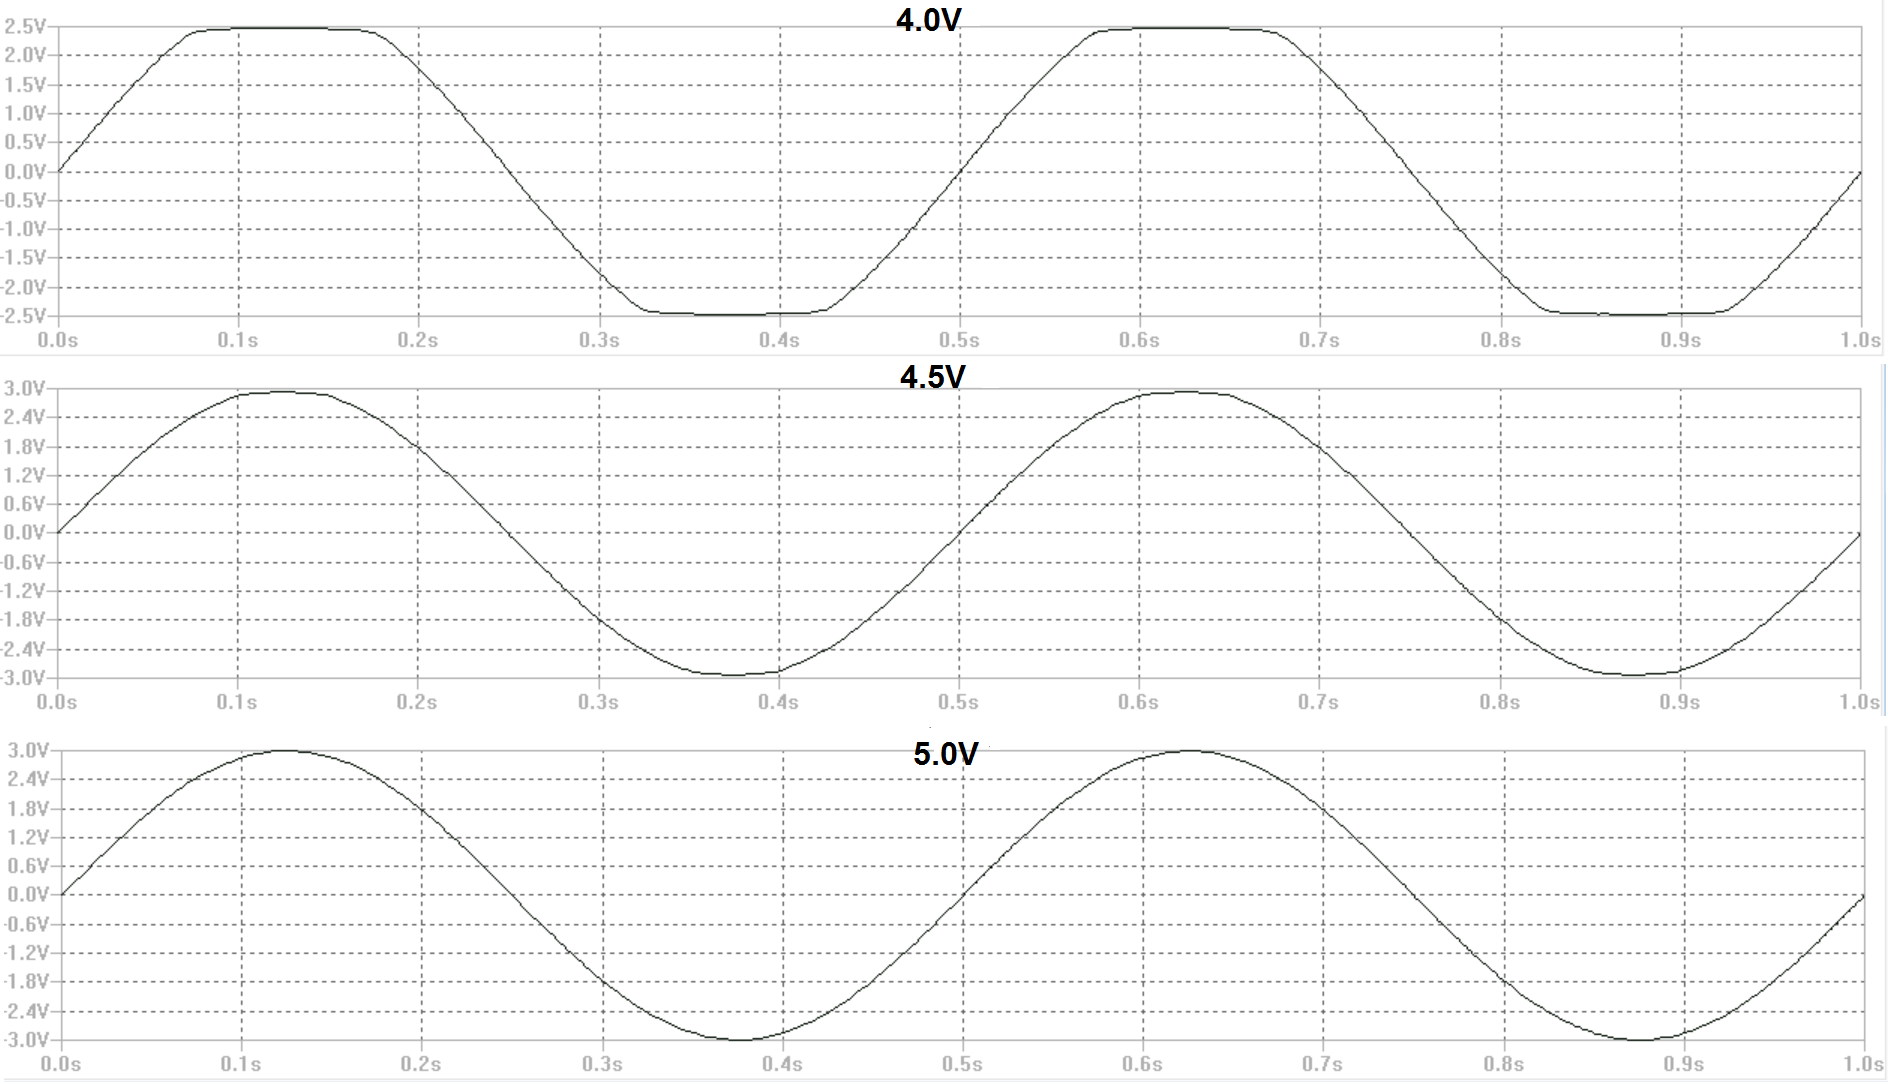
\includegraphics[scale=0.4]{figures/cProblemloesning/Spaendingsforsyning.PNG}
	\caption{Figuren viser simuleringen af spændingsforsyningen ved hhv. $5$V, $4.5$V og $4$V. Det fremgår at figuren at spændingen går i klippet ved ved $4.5$V og går i mætning ved $4$V}
	\label{fig:spaendingsforsyning_graf}
\end{figure}
\begin{figure}[H]
	\centering
	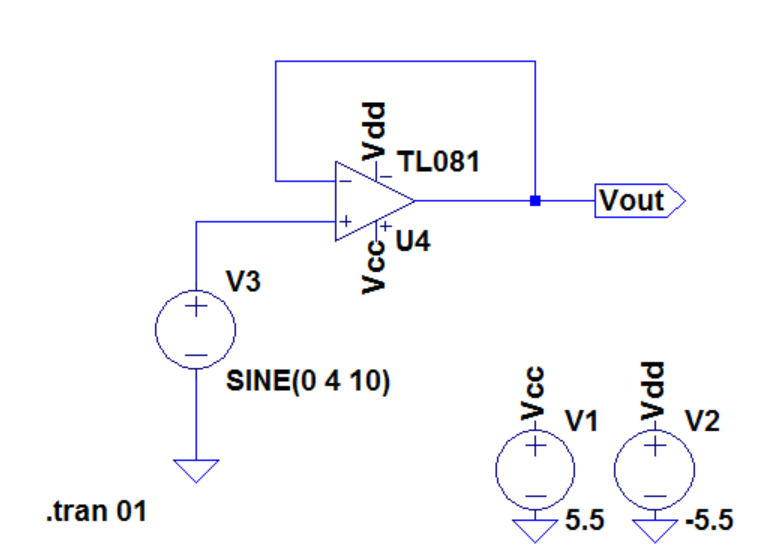
\includegraphics[scale=0.5]{figures/cProblemloesning/Spaendingsforsyning_LTspice.PNG}
	\caption{Figuren viser opbygningen af spændingsforsyningen. Inputsignalet er en sinuskurve. Spændingsforsyningen til operationsforstærkereren er på billedet $\pm5.5$V, hvilket er den spænding der anvendes i systemet.}
	\label{fig:spaendingsforsyning}
\end{figure}
Det fremgår ud fra  at spændingen ved $4.3$V bliver klippet, hvor spændingen går i mætning ved $4$V. 

\subsubsection{Implementering og test}
Der undersøges hvorvidt spændingsregulatoren leverer en spænding på $5.5$V, jævnfør afsnit \ref{Krav_spaending_spicifikt} på side \ref{Krav_spaending_spicifikt}. Derudover skal der testes for hvornår spændingen går i mætning, for at undgå klipning af signalet.

%%%%%%%%%%%%5 SKRIV AFSNIT FÆRDIGT.

Batteriernes levetid undersøges ved at teste, hvor mange ampere systemet bruger. På baggrund af dette vil informationen omkring batteriernes levetid give en estimering af, hvornår de skal udskiftes. Testningen foregår ved en serieforbindelse mellem den negative spændingsforsyning $-V_{cc}$ eller positive spændingsforsyning $+V_{cc}$ og systemet. Selve opsætningen af testen illustreres på %\figref{spaendingsforsyning}.

%%%%%%%%%% TJEK ERIKAS RETTELSER TIL AFSNITTET EFTERFØLGENDE
